\section{Wahl der Architektur und verwendete Technologien}
\label{sec:integration_rl_simulation}

\begin{figure}[htbp]
\centering
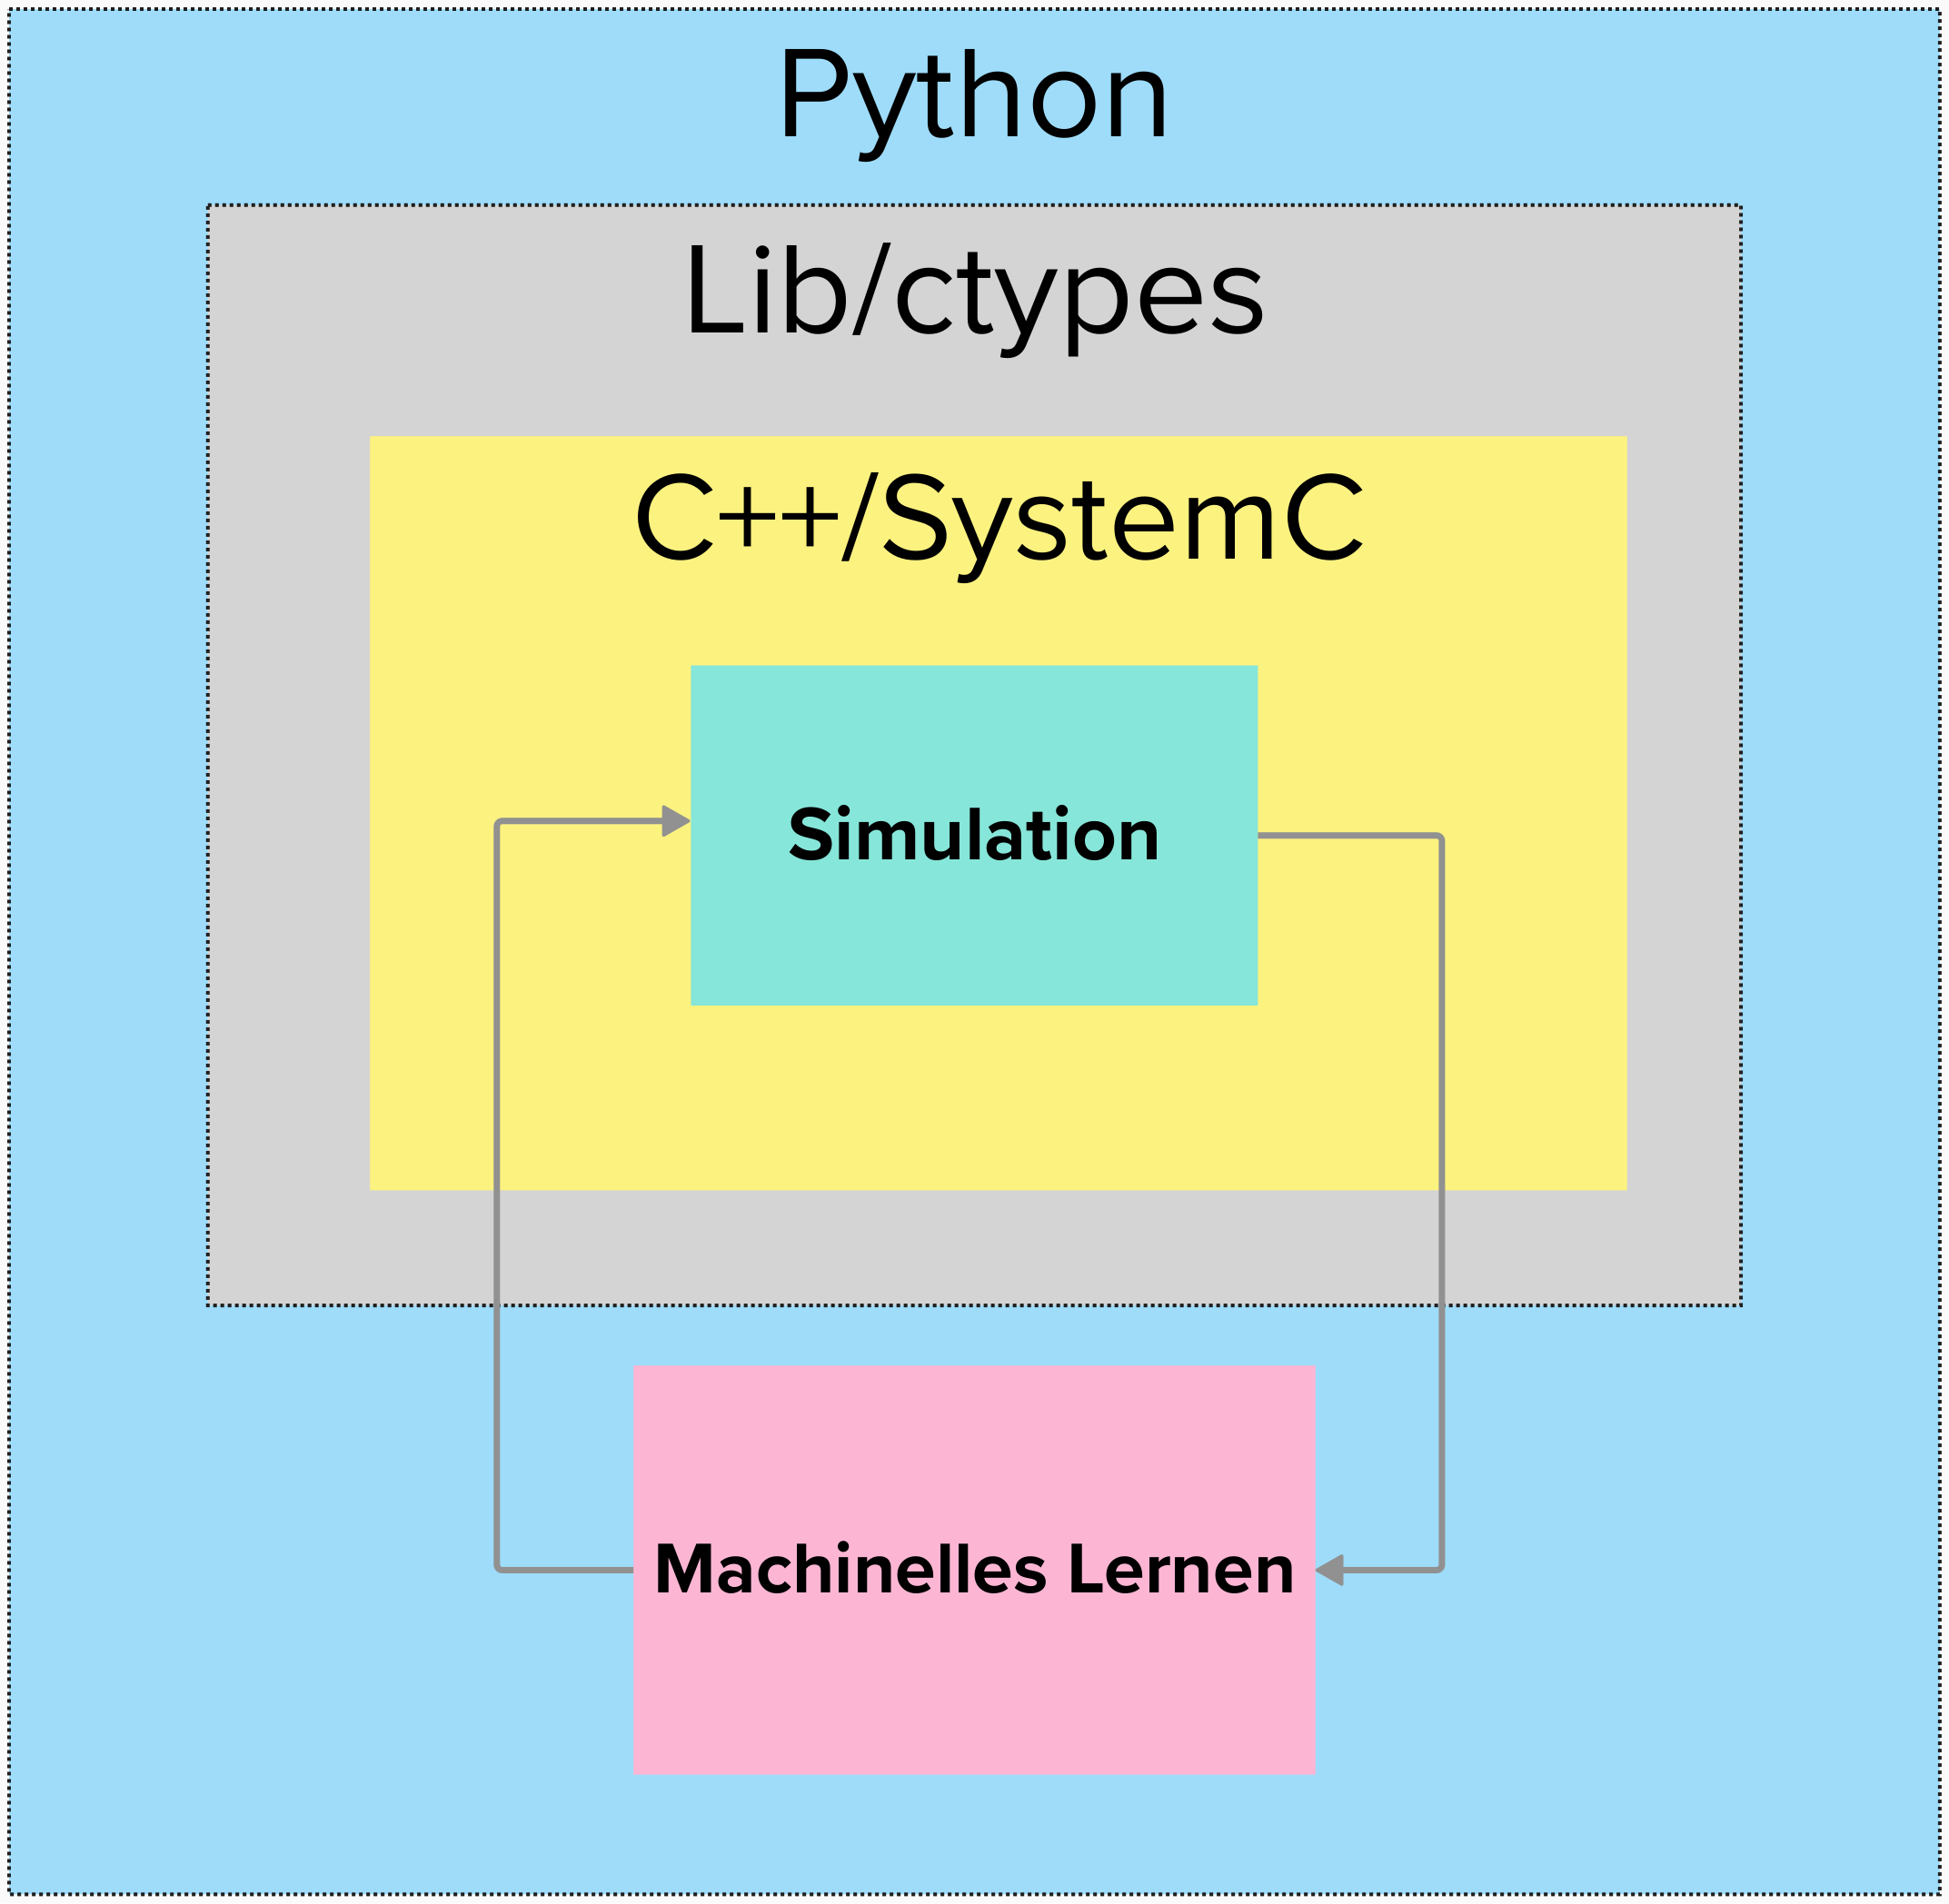
\includegraphics[width=0.4\linewidth]{3Experiment/1SystemC_Wahl_Architectur.png}
\caption{Die Architektur des integrierten Systems, das die Schaltungssimulation und das maschinelle Lernen verbindet.}
\label{fig:integrated_system_architecture}
\end{figure}

Für das Experiment wurden spezifische Technologien und Architekturen ausgewählt, die optimal auf die Anforderungen der Problemstellung abgestimmt sind. Die Entscheidung fiel auf eine Kombination aus Python für die Implementierung des Reinforcement Learning-Teils und SystemC mit C++ für die Simulation der elektronischen Schaltung.

\subsection{Reinforcement Learning mit Python}
Der Reinforcement Learning-Teil des Experiments wurde in Python entwickelt, unter Verwendung von modernen Frameworks wie TensorFlow 2 und Keras. Diese Bibliotheken erleichtern den Entwurf und das Training von neuronalen Netzwerken durch ihre hohe Abstraktion und Benutzerfreundlichkeit. Zusätzlich wurde CUDA verwendet, um das Training der Modelle auf Grafikkarten zu beschleunigen und somit die Konvergenzzeit signifikant zu reduzieren.

\subsection{SystemC und C++ für die Schaltungssimulation}
Der Teil des Experiments, der sich auf die elektronische Schaltung bezieht, wurde in SystemC implementiert, einem C++ basierten Modellierungsframework, das sich durch seine Fähigkeit zur schnellen und präzisen Simulation von Hardwarekomponenten auszeichnet. SystemC bietet eine hohe Modularität und Eignung für die Entwicklung komplexer Schaltungssysteme und ermöglicht eine detaillierte Analyse der Schaltungsverhalten unter verschiedenen Bedingungen.

\paragraph{Integration von Python und SystemC}
Die Integration der in Python entwickelten Reinforcement Learning-Komponente mit der in SystemC implementierten Schaltungssimulation stellt eine besondere technische Herausforderung dar. Diese wurde durch den Einsatz spezialisierter Schnittstellen und Protokolle gemeistert, welche die beiden unterschiedlichen Umgebungen miteinander kompatibel machen und einen reibungslosen Datenaustausch gewährleisten.

\paragraph{Lib/ctypes als Brücke}
Lib/ctypes ist eine Bibliothek in Python, die es ermöglicht, C-Funktionen innerhalb der Python-Umgebung aufzurufen. Dies erlaubt eine effiziente Integration der C++-basierten Schaltungssimulation in das Python-basierte Lernmodell, ohne dass die Leistung darunter leidet.

\paragraph{Modulare und erweiterbare Softwareentwicklung}
Die gesamte Entwicklung folgte den Prinzipien der Kapselung, objektorientierten Programmierung und Interface-gesteuerten Design, was die spätere Anpassung und Erweiterung auf andere Schaltungsmodelle ermöglicht. Dieser modulare Ansatz trägt dazu bei, dass die entwickelten Lösungen auch in anderen Kontexten und für verschiedene Schaltungstypen anwendbar sind.



Für das Kernstück des Experiments, die Wahl der geeigneten Reinforcement Learning-Architektur, fiel die Entscheidung auf den Deep Deterministic Policy Gradient (DDPG). Dieser Ansatz bietet mehrere Vorteile, die ihn für das vorliegende Experiment besonders qualifizieren. Bei der Wahl der Architektur für dieses Experiment wurden drei Hauptgründe berücksichtigt:

\begin{itemize}
    \item Behandlung kontinuierlicher Aktionsräume: Die gewählte Architektur kann effektiv mit kontinuierlichen Aktionsräumen umgehen, was für analoge Anwendungen und reale Einsatzgebiete entscheidend ist.
    \item Schnelle Konvergenz: Der Deep Deterministic Policy Gradient (DDPG) zeichnet sich durch seine schnelle Konvergenz aus. Da die Simulationen im Experiment zeitaufwendig sind, ist eine zügige Konvergenz wichtig für die Effizienz des Trainingsprozesses.
    \item Modularität der Architektur: Die aus Äktor (Actor) und Kritiker (Critic) bestehende Architektur ermöglicht eine Variation von Gewichten und Schichten in getrennten Netzwerkteilen, was besonders bei der Übertragung des Modells auf physische Implementierungen wie einen Mikrochip von Vorteil ist.
\end{itemize}

Die Architektur wurde also aufgrund ihrer Eignung für kontinuierliche Aktionsräume, ihrer schnellen Konvergenz und ihrer Modularität ausgewählt, um den Anforderungen des Experiments gerecht zu werden.
